\section{Prezentacja warstwy użytkowej projektu}
\subsection{Interfejs użytkownika}
System rezerwacji lotów oferuje trzy główne interfejsy:
\begin{itemize}
\item \textbf{Ekran logowania i rejestracji} - dla użytkowników
\item \textbf{Ekran klienta} - do przeglądania dostępnych lotów, rezerwacji biletów
\item \textbf{Panel klienta} - do zarządzania rezerwacjami oraz przeglądania danych
\end{itemize}

\begin{figure}[H]
\centering
\begin{subfigure}{0.45\textwidth}
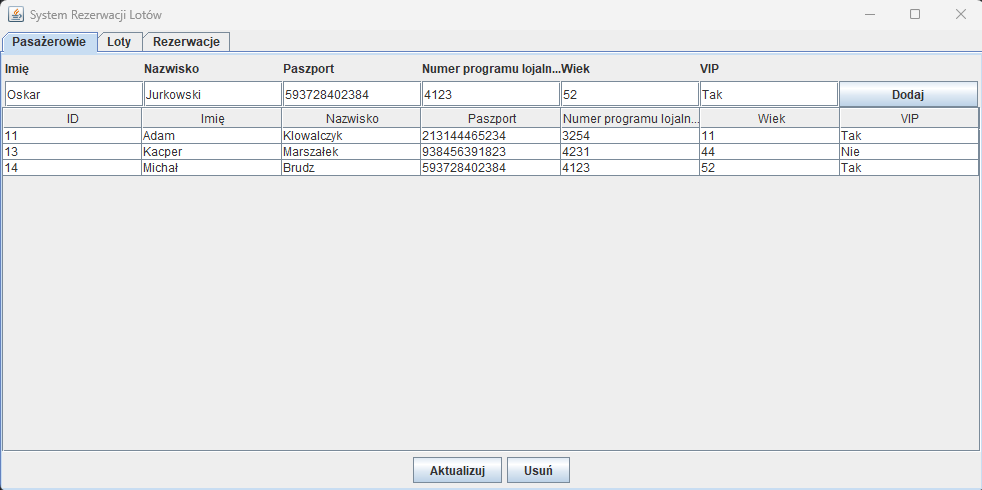
\includegraphics[width=\textwidth]{figures/1.png}
\caption{Ekran główny - przegląd pasażerów}
\label{fig:main_screen}
\end{subfigure}
\begin{subfigure}{0.45\textwidth}
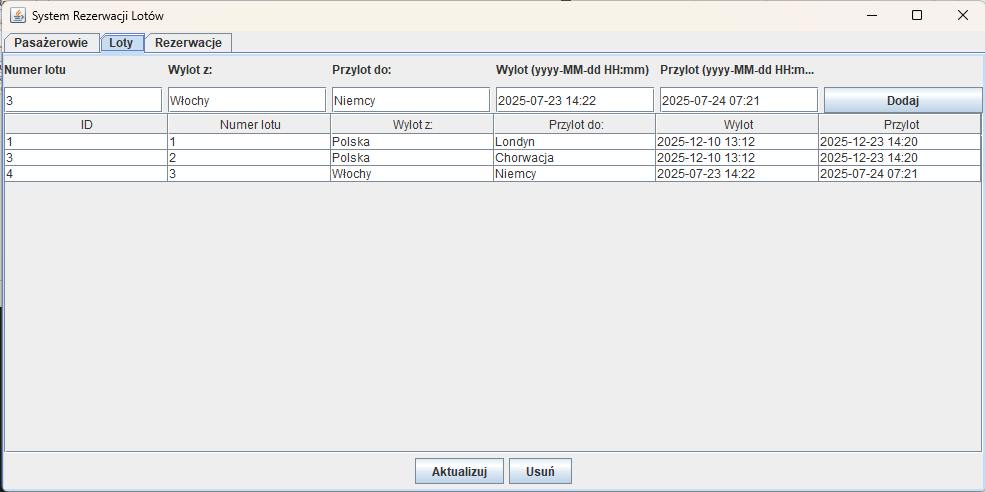
\includegraphics[width=\textwidth]{figures/2.png}
\caption{Ekran z listą lotów}
\label{fig:flights_screen}
\end{subfigure}
\caption{Podstawowe ekrany systemu rezerwacji lotów}
\end{figure}

\subsection{Interfejs logowania}
System oferuje ekran logowania, na którym użytkownik wprowadza swój login oraz hasło. W przypadku braku konta, użytkownik może przejść do ekranu rejestracji, gdzie może stworzyć nowe konto.

\begin{figure}[H]
\centering
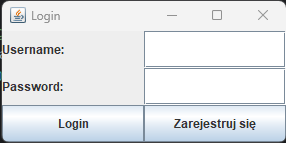
\includegraphics[width=0.45\textwidth]{figures/4.png}
\caption{Ekran logowania}
\label{fig:login_screen}
\end{figure}

Po pomyślnym zalogowaniu, użytkownik zostaje przeniesiony do ekranu głównego, gdzie może przeglądać dostępne loty, rezerwować bilety oraz zarządzać swoimi danymi.

\subsection{Rejestracja użytkownika}
W przypadku braku konta, użytkownik może zarejestrować się poprzez formularz rejestracyjny, gdzie wprowadza dane takie jak login, adres e-mail, hasło oraz jego potwierdzenie.

\begin{figure}[H]
\centering
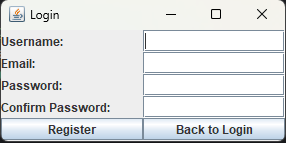
\includegraphics[width=0.45\textwidth]{figures/5.png}
\caption{Ekran rejestracji użytkownika}
\label{fig:register_screen}
\end{figure}

\subsection{Przepływ użytkownika}
Typowy scenariusz użycia systemu:
\begin{enumerate}
\item Użytkownik uruchamia aplikację i loguje się na swoje konto.
\item Po zalogowaniu użytkownik przegląda dostępne loty.
\item Wybiera lot, uzupełnia dane pasażera, a następnie rezerwuje bilet.
\item Użytkownik może również edytować swoje dane lub sprawdzić historię rezerwacji.
\end{enumerate}

\subsection{Panel klienta}
Panel klienta jest dostępny po zalogowaniu się na konto użytkownika. W panelu klienta użytkownik może zarządzać swoimi rezerwacjami, przeglądać historię oraz edytować swoje dane.

\begin{figure}[H]
\centering
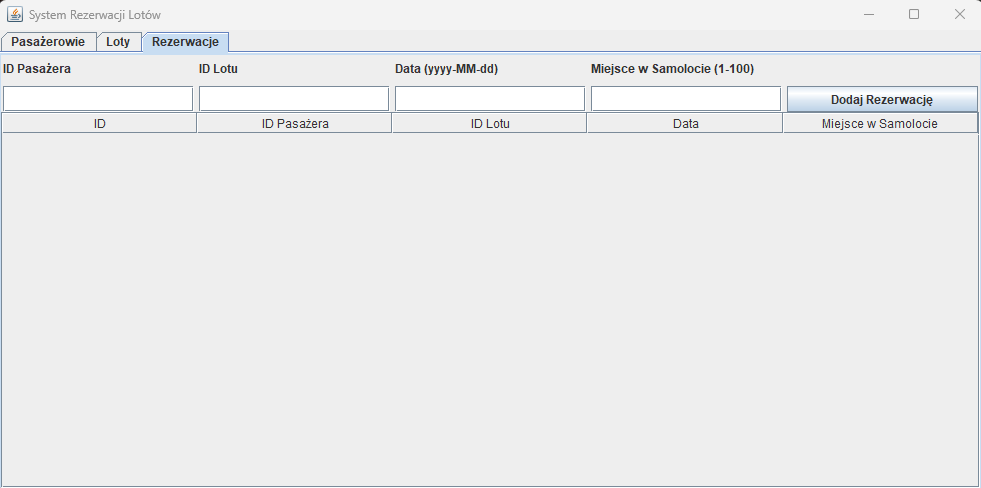
\includegraphics[width=0.7\textwidth]{figures/3.png}
\caption{Panel klienta systemu rezerwacji}
\label{fig:client_panel}
\end{figure}

Funkcjonalności panelu klienta:
\begin{itemize}
\item \textbf{Zarządzanie rezerwacjami} - przeglądanie, edytowanie i anulowanie rezerwacji.
\item \textbf{Przegląd danych osobowych} - możliwość edytowania danych pasażera.
\item \textbf{Historia rezerwacji} - monitorowanie rezerwacji dokonanych przez użytkownika.
\end{itemize}
